\documentclass[a4paper,12pt]{article}
\usepackage[a4paper, total={180mm, 272mm}]{geometry}

\usepackage{fontspec}
\setmainfont[Path=fonts/, Extension=.ttf]{ipaexm}

\setlength\parindent{3.5em}
\setlength\parskip{0em}
\renewcommand{\baselinestretch}{1.247}

\usepackage{eepic}

\usepackage{tikz}

\begin{document}

\thispagestyle{empty}

\Large
\noindent \\
Level Auto Ino\medskip
\par
\normalsize
絵の明るさのレンジを最大に広げます。\\
\par
暗いマスク用画像を明るくする等の自動的な level 補正をします。\\
\par
入力画像の最も暗い値と最も明るい値を元にして、数値として最\par
も暗い値(Out Min)と最も明るい値(Out Max)に明るさのレンジを\par
広げます。\par
-{-}> \textquotedbl Level Auto 図1 計算図\textquotedbl 参照\\
\par
RGBA チャンネル各々にレンジを広げるので、RGBA のバランスはと\par
りません。そのため色の付いた画像は色が変わることがあります\par
ので注意してください。\\
\par
結果をチェックするときは、サブカメラを使わないでください。\par
サブカメラは入力画像の範囲が違うため、入力画像の最暗値と最\par
明値が変わり、正確な処理ができません。\\
\\
-{-}- \ 入力 \ -{-}-\\
Source\par
処理をする画像を接続します。\\
\\
-{-}- \ 設定 \ -{-}-\\
In Min Shift\\
In Max Shift\par
入力画像 Pixel の最小値と最大値は、自動的に計算しますが、その\par
値に加算して調整します。\par
例えば一ヶ所だけ明るい Pixel があってそれを無視したいとき、\par
\textquotedbl In Max Shift\textquotedbl にマイナスを指定することでレンジをひろげます。\par
Pixel 値(8 or 16bits)をゼロから1の値として指定します。\par
最小は-1、最大は1です。\par
\noindent \hskip 7em Min \ \ \ \ \, 0\par
\noindent \hskip 7em Max \ \ \ \ -1\par
だと画面は真っ暗になります。\par
\noindent \hskip 7em Min \ \ \ \ \, 1\par
\noindent \hskip 7em Max \ \ \ \ \ 0\par
とすると、画面は真っ白になります。\par
0とすれば shift による調整はありません。\par
初期値は両方とも0です。\\
\\
Out Min

\newpage

\thispagestyle{empty}

\ \vspace{-0.2em}
\par
\noindent Out Max\par
出力画像の最も暗い値(最小値)と最も明るい値(最大値)を決定し\par
ます。\par
最小は0、最大は1です。\par
初期値は\par
\noindent \hskip 7em Out Min が0\par
\noindent \hskip 7em Out Max が1\par
です。\\
\\
Gamma\par
\textquotedbl Out Min\textquotedbl と\textquotedbl Out Max\textquotedbl の間で gamma 補正します。\par
0.1から1.0の間だと、画像が暗くなります。\par
1.0を指定すると補正しません。\par
1.0から10.0の間では、明るくなります。\par
初期値は1です。\\
\\
Level Auto 図1 \ \ 計算図

\large
\noindent \begin{picture}(0,0)
\linethickness{0.01em}
\put(18.5,-94){\line(0,-1){81}}
\put(18.5,-94){\line(-2,-3){4}}
\put(18.5,-94){\line(2,-3){4}}
\put(18.5,-175){\line(-2,3){4}}
\put(18.5,-175){\line(2,3){4}}

\put(114,-22){\line(0,-1){199}}
\put(256,-22){\line(0,-1){199}}
\put(85,-51){\line(1,0){199}}
\put(85,-193){\line(1,0){199}}

\put(101,-7){\small{IN}}
\put(233,-7){\small{OUT}}
\put(290,-51){\small{1}}
\put(290,-193){\small{0}}
\put(72,-91){\small{max}}
\put(258,-69){\small{max}}
\put(116,-105){\small{max\_shift}}
\put(116,-176){\small{min\_shift}}
\put(72,-188){\small{min}}
\put(258,-188){\small{min}}
\end{picture}\\[3em]

\noindent \hskip 3.8em 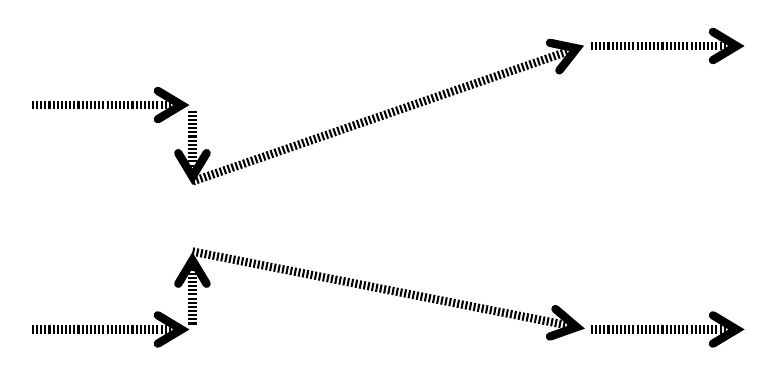
\begin{tikzpicture}[line width=3pt]
\draw[line cap=round] (1.6,-0.75) -- (1.9,-0.93) -- (1.6,-1.11);
\draw[dashed,dash pattern=on 0.75pt off 0.75pt] (0,-0.93) -- (1.9,-0.93);

\draw[line cap=round] (8.65,0) -- (8.95,-0.18) -- (8.65,-0.36);
\draw[dashed,dash pattern=on 0.75pt off 0.75pt] (7.1,-0.18) -- (8.95,-0.18);

\draw[line cap=round] (1.6,-3.6) -- (1.9,-3.78) -- (1.6,-3.96);
\draw[dashed,dash pattern=on 0.75pt off 0.75pt] (0,-3.78) -- (1.9,-3.78);

\draw[line cap=round] (8.65,-3.6) -- (8.95,-3.78) -- (8.65,-3.96);
\draw[dashed,dash pattern=on 0.75pt off 0.75pt] (7.1,-3.78) -- (8.85,-3.78);

\draw[line cap=round] (1.86,-1.54) -- (2.04,-1.84) -- (2.22,-1.54);
\draw[dashed,dash pattern=on 0.75pt off 0.75pt] (2.04,-1) -- (2.04,-1.84);

\draw[line cap=round] (1.86,-3.2) -- (2.04,-2.9) -- (2.22,-3.2);
\draw[dashed,dash pattern=on 0.75pt off 0.75pt] (2.04,-2.9) -- (2.04,-3.74);

\draw[line cap=round] (6.58,-0.14) -- (6.92,-0.21) -- (6.7,-0.49);
\draw[dashed,dash pattern=on 0.75pt off 0.75pt] (2.04,-1.9) -- (6.92,-0.21);

\draw[line cap=round] (6.65,-3.52) -- (6.92,-3.75) -- (6.58,-3.87);
\draw[dashed,dash pattern=on 0.75pt off 0.75pt] (2.04,-2.79) -- (6.92,-3.75);

\end{tikzpicture}

\end{document}